\documentclass{article}%You can define the type of paper here.
%%Useful packages that I commonly use.
\usepackage[numbers]{natbib}%Bibliography package (help at http://merkel.zoneo.net/Latex/natbib.php).
\usepackage{url}%Package to highlight url.
\usepackage{times}%Sets font to be times.
\usepackage{siunitx}
\usepackage{alltt}%Allows the use of verbatim (good for printing out code).
\usepackage{graphicx}%Used to import images.
\usepackage{amsmath, amssymb, amscd}%Contains the AMS expanded math symbols library.
\usepackage{algorithm, algorithmic} %pseudo-code
%%For those who want smaller margins, you can use this:
\usepackage[top=1in, bottom=1in, left=1in, right=1in]{geometry}

\begin{document}

%%Title

\title{Firn Densification Model}
\author{Cummings, Evan \and Davis, Tyler \and Brinkerhoff, Douglas}
\maketitle
\begin{center}
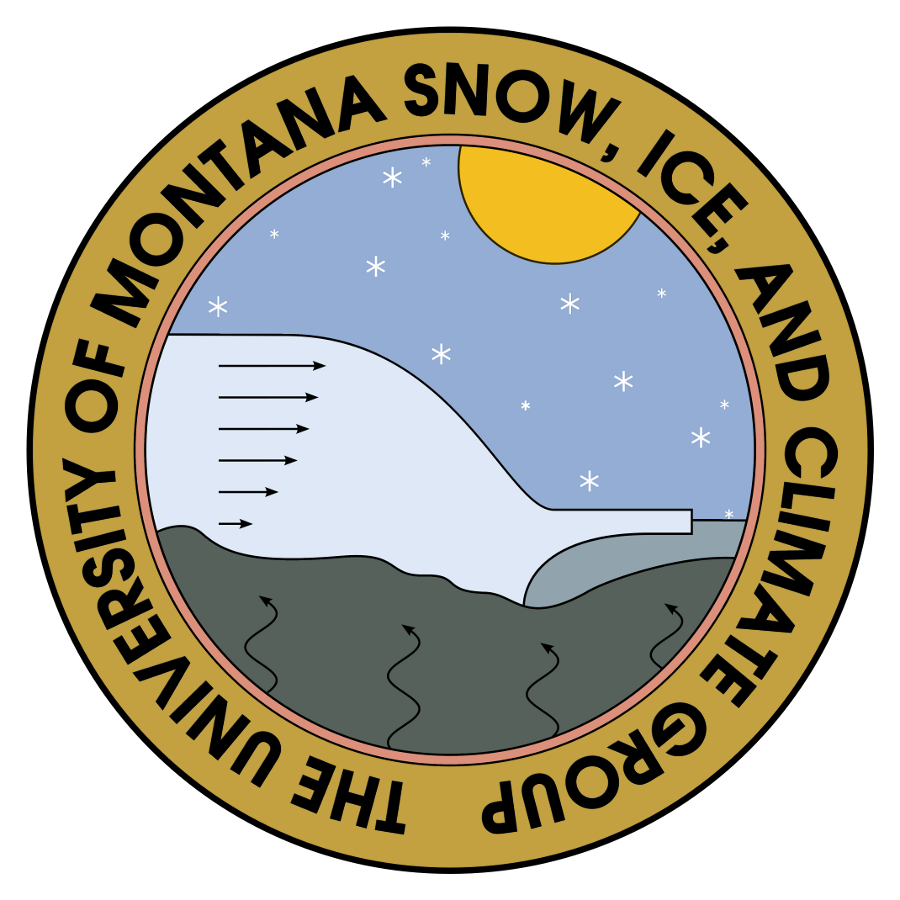
\includegraphics[width=0.45\textwidth]{images/logo.png}
\end{center}

%%Makes the paper use two columns
\twocolumn

%%Introduction =================================================================
\section{Introduction}

The top layer of snow on a glacier or ice sheet increases in density as depth increases.  Several models have been created to simulate this process, some based on temperature and others based on enthalpy.  I have re-created these models with the finite-element software package FEniCS.

%% Temperature =================================================================
\section{Temperature Solution}

We begin with the standard heat-transport equation (Patterson, 2001

  $$
  \rho c_i \frac{\partial T}{\partial t} = 
    k_i \frac{\partial^2 T}{\partial z^2} +
    \left( \frac{dk}{dt} - \rho c_i w \right) \frac{\partial T}{\partial z}
  $$
with heat sources from the deformation of ice ommitted, $\rho$ density, $c_i$ heat capacity, $k_i$ thermal conductivity, $w$ vertical velocity, and $T$ temperature of firn.  We can descritize the temperature differential with the second-order accurate backward-difference formula
  $$\frac{\partial T}{\partial t} = \frac{T^{k-2} - 4T^{k-1} + 3T}{2dt},$$
with superscripts referring to time index.
To solve the total derivative $dk/dt$ we must apply the chain rule
  $$
  \frac{dk_i}{dz} = 
  \frac{\partial k_i}{\partial \rho} \frac{\partial \rho}{\partial z} + 
  \frac{\partial k_i}{\partial T} \frac{\partial T}{\partial z}.
  $$
The thermal conductiviy of ice is defined by Arthern et. al, 1998 as
  $$k_i = 2.1 \left(\frac{\rho}{\rho_i}\right)^2,$$
and gives
  $$
  \frac{\partial k_i}{\partial \rho} = 
    4.2 \frac{\rho}{\rho_i^2}
  $$
and
  $$
  \frac{\partial k_i}{\partial T} = 
    \frac{4.2}{\rho_i^2} \left( \frac{\partial \rho}{\partial T} \right).
  $$
Patterson, 2001 defined 
  $$
  \frac{\partial \rho}{\partial T} = 
    \SI{5.6e-2} \exp ((\SI{-5.7e-3})T).
  $$
The vertical velocity of ice, $w$, is directly proportional to the accumulation, $b$,
  $$
  w = -\frac{b}{\rho}
  $$
with $b$ in units of $kg\ m^{-2}\ s^{-1}$.  The densification process is defined with the material derivative
  $$\frac{d \rho}{dt} = \frac{\partial \rho}{\partial t} + 
    w\frac{\partial \rho}{\partial z}.$$
We again descritize the time partial with the backward-difference formula :
  $$\frac{\partial \rho}{\partial t} = 
      \frac{\rho^{k-2} - 4\rho^{k-1} + 3\rho}{2dt}.$$
Arthern et. al, 2010 described the total derivative with the formula  
  $$
  \frac{d \rho}{dt} = 
  \begin{cases}
   c_0(\rho_i - \rho), &\rho <= 550\ kg\ m^{-3}\\
   c_1(\rho_i - \rho), &\rho > 550\ kg\ m^{-3}
  \end{cases}$$
Zwally and Li, 2002 defined the multiplying constant $c$ with an arrhenius-type relation
  $$
  c_0 = c_1 = 
  b \rho_i / \rho_w \beta(T)K_{0G}(T)\exp \left( -\frac{E(T)}{RT} \right),
  $$
with $K_{0G}(T) \exp(-E(T)/(RT)) = 8.36T^{-2.061}$, and $\beta(T)$ a smoothing function to match a desired density rate.  Arthern et. al 2010 developed a semi-empirical formula by coupling the rate equations for Nabarro-Herring creep and normal grain-growth : 
  $$
  \begin{cases}
    c_0 = M_0 bg\frac{k_{c0}}{k_g}\exp\left(\frac{E_c}{RT} + 
          \frac{E_g}{RT_{avg}}\right)\\
    c_1 = M_1 bg\frac{k_{c1}}{k_g}\exp\left(\frac{E_c}{RT} + 
          \frac{E_g}{RT_{avg}}\right)
  \end{cases},
  $$
with the creep coefficients defined as
  $$
  \begin{cases}
    k_{c0} = \SI{9.2e-9} m^3\ s\ kg^{-1} \\
    k_{c1} = \SI{3.7e-9} m^3\ s\ kg^{-1}  
  \end{cases}
  $$
and $M$ defined by Ligtenberg et. al 2011 to better fit with observed densification rates in higher-temperature environments :
  $$
  \begin{cases}
    M_0 = 2.366 - 0.293\ln(b*\SI{1e3})\\
    M_1 = 1.435 - 0.151\ln(b*\SI{1e3})
  \end{cases}.
  $$
Ligtenberg et. al 2011 developed a firn surface density expression from data :
  $$ \rho_s = -151.94 + 1.4266(73.6 + 1.06T_s + 0.0669A + 4.77V_a).$$




%% Enthalpy ====================================================================
\section{Enthalpy Solution}
	$$
  \rho \frac{dH}{\partial t} = \frac{\partial}{\partial z} 
    \left( 
      \begin{Bmatrix}
        K_i(H) \\
        K_0
      \end{Bmatrix}
      \frac{\partial H}{\partial z} 
    \right)
  $$
  $$K_i(H) = \frac{k_i}{c_i}$$
  $$K_0 = \frac{K_i(H)}{10}$$
  $$\frac{d \rho}{dt} = \frac{\partial \rho}{\partial t} + 
    w\frac{\partial \rho}{\partial z}$$
  $$\frac{d \rho}{dt} = c(\rho_i - \rho)$$
  $$c = M_Obg\frac{k_c}{k_g}\exp\left(\frac{E_c}{RT} + 
    \frac{E_g}{RT_{avg}}\right)$$
  $$
  k_c =
  \begin{cases}
    \SI{3.7e-9}, &\rho > 550\ kg\ m^{-3}\\
    \SI{9.2e-9}, &\rho <= 550\ kg\ m^{-3}
  \end{cases}
  $$
  $$
  M_O =
  \begin{cases}
    2.366 - 0.293\log A, &\rho > 550\ kg\ m^{-3} \\
    1.435 - 0.151\log A, &\rho <= 550\ kg\ m^{-3}
  \end{cases}
  $$
  $$k_i = 2.1 \left(\frac{\rho}{\rho_i}\right)^2$$
  $$c_i(T) = 146.3 + 7.253 T $$
  $$w(z) = - \frac{b}{\rho}$$
  $$H = c_i(T_w - T_0) + \omega L_f,  \text{where } H > H_{sp}$$
  $$\omega L_f = H - c_i(T_w - T_0)$$
  $$T = \frac{H}{c}$$
  $$l_{n+1} = l_n \frac{\rho_{ini}}{\rho}$$
  $$s_{n} = (z_s - z_b) \frac{s_{n-1} - z_b}{z_{s} - z_b} + w_s dt $$


%%Method-----------------------------------------------------------------------
\section{Method}

The implicit method used by the numerical method of lines to solve PDEs uses the future to predict the future.  First the diffusion term:

$$\frac{k}{\rho C_p} \frac{\partial ^2 \theta(x, z, t)}{\partial z^2}.$$

\noindent After discretization this becomes

$$\frac{k}{\rho C_p} \frac{u_{j+1}^n - 2u_j^n + u_{j-1}^n}{\Delta z^2},$$

where $j$ is the z-position and $n$ is the time-position.\\
\\
\noindent This can be represented as a matrix as

$$\mathbf{A} = 
\begin{bmatrix}
  0 &0 &0 &0 &\cdots &\cdots &0 \\
  \alpha &-2\alpha &\alpha &0 &\cdots &\cdots &0 \\
  0 &\alpha &-2\alpha &\alpha & \cdots &\cdots &0 \\
  &\ddots & \ddots &\ddots  & & & \\
  \vdots &\cdots &\alpha &-2\alpha &\alpha  &\cdots &\vdots \\
  & & &\ddots &\ddots &\ddots &\\
  0 & \cdots &\cdots &0 &\alpha &-2\alpha &\alpha \\
  0 & \cdots &\cdots &0 &0 &0 &0 \\
\end{bmatrix},$$

where $\alpha = \frac{k}{\rho C_p \Delta z^2}$.\\
\\
\noindent Now for the vertical advection term :

$$w(z)\frac {\partial \theta}{\partial z}.$$

\noindent Taking the velocity to be positive and into the column of ice, this becomes

$$w(z)\frac{-3u_{j}^n + 4u_{j+1}^n - u_{j+2}^n}{2\Delta z},$$

which can be represented as a matrix as:

$$w(z)\mathbf{B} = 
\begin{bmatrix}
  1 &0 &0 &0 &\cdots &\cdots &0 \\
  -3\beta &4\beta &-\beta &0 &\cdots &\cdots &0 \\
  0 &-3\beta &4\beta &-\beta & \cdots &\cdots &0 \\
  &\ddots & \ddots &\ddots  & & & \\
  \vdots &\cdots &-3\beta &4\beta &-\beta  &\cdots &\vdots \\
  & & &\ddots &\ddots &\ddots &\\
  0 & \cdots &\cdots &0 &-3\beta &4\beta &-\beta \\
  0 & \cdots &\cdots &0 &0 &0 &1 \\
\end{bmatrix},$$

where $\beta = \frac{1}{2\Delta z}$ and $w(z)$ is a vector with its length 
\indent equal to the number of nodes.\\
\\
\newpage

\noindent The values for horizontal advection and heat sources from the deformation of ice can be calculated directly without the need for a matrix.  

The surface temperature can be designated any value desired, here a function:

$$\theta(z_s) = -10 + 5 \sin\left(2\pi \frac{t}{spy}\right),$$

where $spy$ is the number of seconds in a year.\\
\\
\noindent Geothermal heat flow can be described with

$$k \frac{\partial \theta}{\partial z} \Bigr\rvert_{z=z_b}= -Q_{geo},$$

where 
\begin{align*} 
  \frac {\partial \theta}{\partial z} &= 
    \frac{u_{j-2}^n - 4u_{j-1}^n + 3u_{j}^n}{2\Delta z},
  \\
  Q_{geo} &= 42.0 \times 10^{-3} \left( \frac Km \right),
\end{align*}

and solving for $u_j$ on the bottom results in

$$u_{j}^n = \frac 13 \left( \frac{-2\Delta z Q_{geo}}{k} + 4u_{j-1}^n - u_{j-2}^n\right).$$

\noindent Under the pressure of the column of ice the melting point may drop below $0^\circ C$.  This pressure melting point of ice is defined as

$$\theta_{PMP} = \beta \rho g (z_s - z_b)\ \textnormal{in }^\circ C,$$

where $g \approx 9.81 \frac {m}{s^2}$ is the acceleration of gravity and $\beta = 9.8 \times 19^{-8} \frac{K}{Pa}$ is the pressure dependence of the melting point.  Because ice and water maintain the same temperature while undergoing a change of phase, $\theta_{PMP}$ is the maximum temperature that the ice can reach.
 
Utilizing Python's sparse matrix package simplifies the creation of the $\mathbf{A}$ and $\mathbf{B}$ matrices.  Once these are created and the variables and constants defined, python's ODE integrator VODE in 'BDF' mode can be efficiently used to calculate $\theta$ for each time-step.  VODE requires the right-hand-side function just described:

\begin{algorithm}
  \caption{Right-hand-Side Function}
  \begin{algorithmic} 
%  \STATE \textbf{INPUTS}: 
%  \STATE \ \ \ $t$ - current time, $\vec \theta$ - temperature of ice 
%    column, 
%  \STATE \ \ $\vec w$ - vertical ice velocity, $\vec u$ - horizontal ice 
%    velocity, 
%  \STATE \ \ $\frac{\partial \theta}{\partial x}$ - horizontal temp.
%     gradient, $\vec \phi$ - deformation heat, 
%  \STATE \ \ \ $\rho$ - ice density, $C_p$ - heat capacity of ice 
%  \STATE \ \ \ $Q_{geo}$ - geothermal heat flux, 
%  \STATE \ \ \ $\theta_{PMP}$ - pressure melting point of ice
%  \STATE \ \ \ $\mathbf{A}$ - diffusion matrix, 
%    $\mathbf{B}$ - vertical advection matrix, 
%  \STATE \textbf{OUTPUTS}: 
%  \STATE \ \ \ $\vec \theta$ - temperature of ice at next 
%    time-step
    \STATE $\theta_{z_b} := \frac 13 \left( \frac{-2\Delta z Q_{geo}}{k} 
      + 4\theta_{z_b-1} - \theta_{z_b-2}\right)$
    \STATE $\vec \theta := \mathbf{A}\vec \theta - 
      \vec w \mathbf{B}\vec \theta - 
      \vec u \frac{\partial \theta}{\partial x} + 
      \frac{\vec \phi}{\rho C_p}$
    \FOR {$i:=0$ to $z_b$}
      \IF{ $\theta_{z_i} \geq \theta_{PMP}$}
        \STATE $\theta_{z_i} := \theta_{PMP}$
      \ENDIF
    \ENDFOR
    \RETURN $\vec \theta$
  \end{algorithmic}
\end{algorithm}

\newpage
\noindent Here is the equivalent of Algorithm 1 in python code:
\footnotesize
\begin{alltt}
def rhs(t, y):
  # heat flow from bed
  y[-1] = (-Qgeo*2*dz/k + 4*y[-2] - y[-3])/3.0
  # set max temp :
  for i in range(n):
    if y[i] >= Tpmp :
      y[i] = Tpmp
  y = A*y - w*(B * y) - u*dTdx + phi/(rho * cp)
  return y
\end{alltt}
\normalsize
\noindent \textbf{Note}: The extra variables used are defined globally, and therefore are not needed in the parameter list.


%%Verification-----------------------------------------------------------------
\section{Verification of Program}
Using the values given in the previous two sections results in these figures :

\begin{figure}[H]
	\centering
		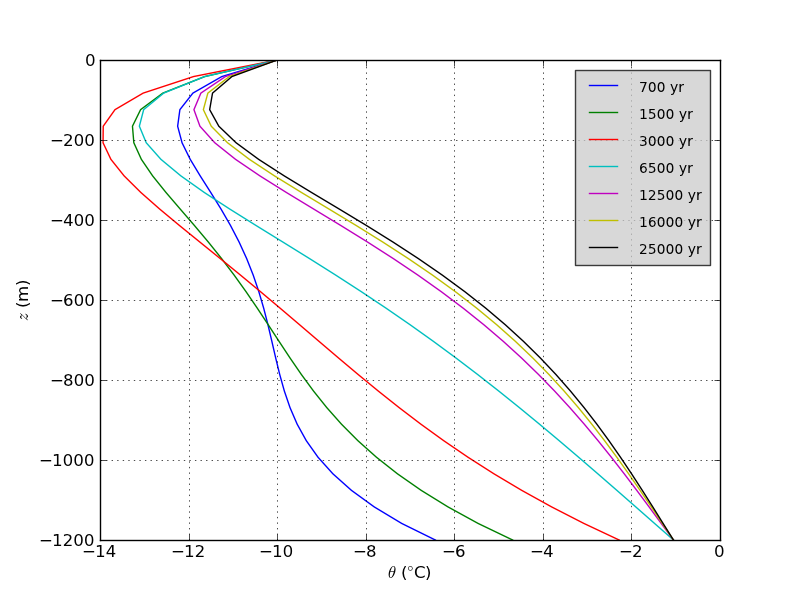
\includegraphics[width=0.45\textwidth]{images/30000yr_converge.png}
	\label{fig:orbits}
	\caption{Temperatures of Ice in 30,000 Years.}
\end{figure}

\begin{figure}[H]
	\centering
		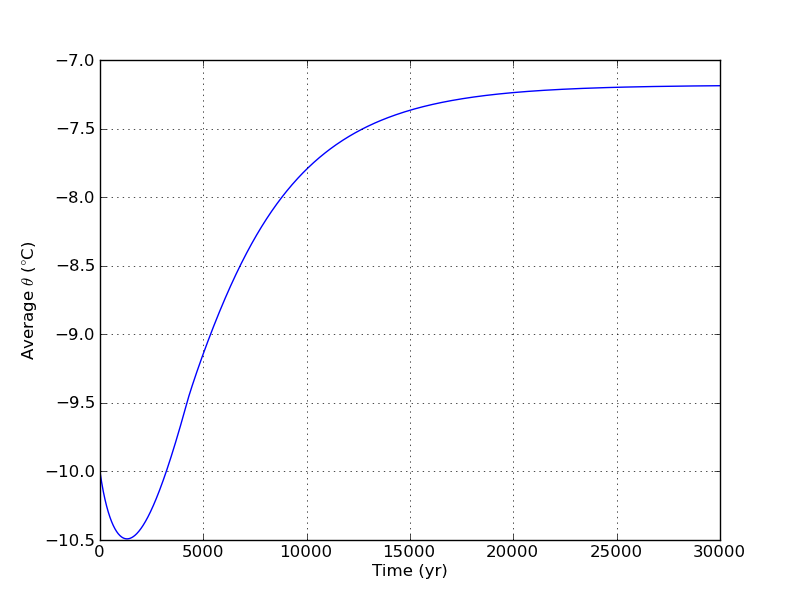
\includegraphics[width=0.45\textwidth]{images/30000yr_avg.png}
	\label{fig:500 year orbit}
	\caption{Average Temperature of Ice in 30,000 Years.}
\end{figure}

\noindent These data show that the temperature finds an equilibrium in around 25,000 years.

\newpage

\noindent To find the maximum depth where melting occurs, it is necessary to zoom into the region on the surface :

\begin{figure}[H]
	\centering
		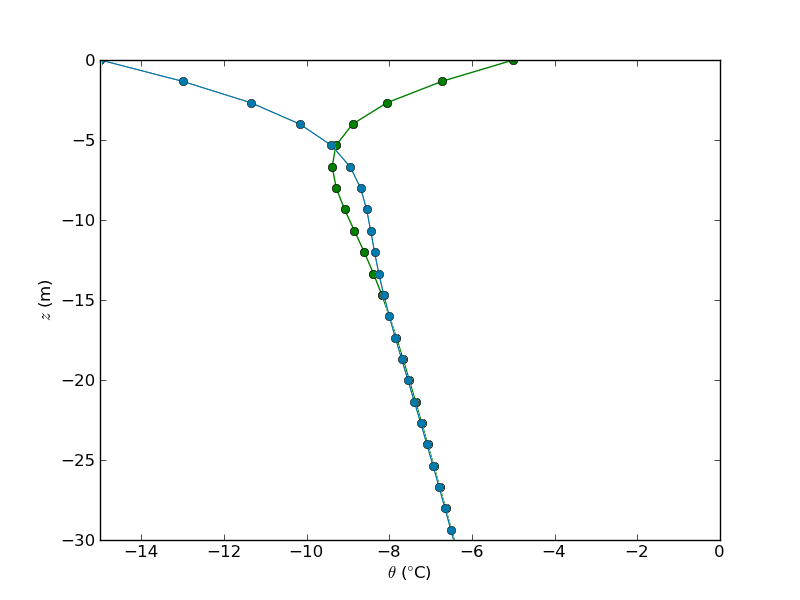
\includegraphics[width=0.42\textwidth]{images/yearHighLow.png}
	\label{fig:500 year orbit}
	\caption{Annual Low and High Temperatures.}
\end{figure}

\noindent These data show that the temperature of the ice stays roug-
hly constant around -16 meters.  Figures 4 and 5 show the results after biasing the temperature by $+15\ ^\circ C$ :

\begin{figure}[H]
	\centering
		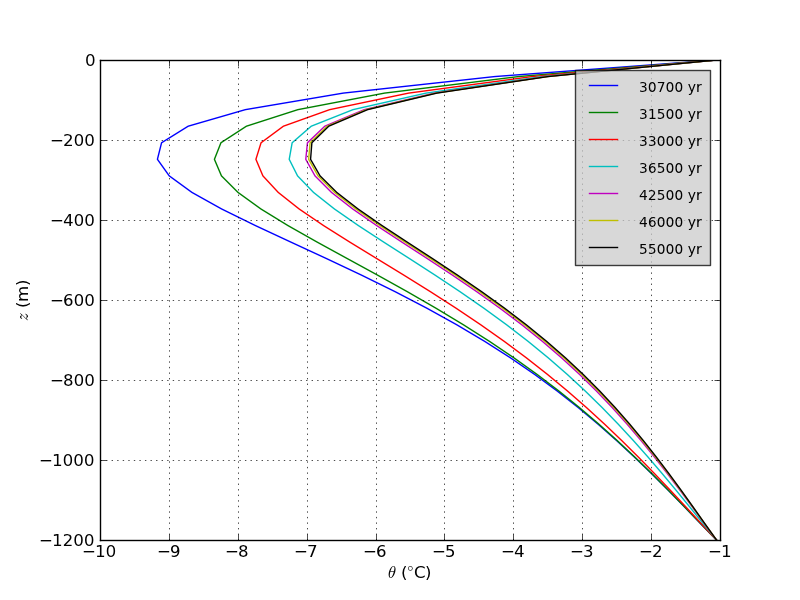
\includegraphics[width=0.42\textwidth]{images/60000yr_converge.png}
	\label{fig:500 year orbit}
	\caption{Temperature of Ice after Biasing the Temperature by $+15\ ^\circ C$}
\end{figure}

\begin{figure}[H]
	\centering
		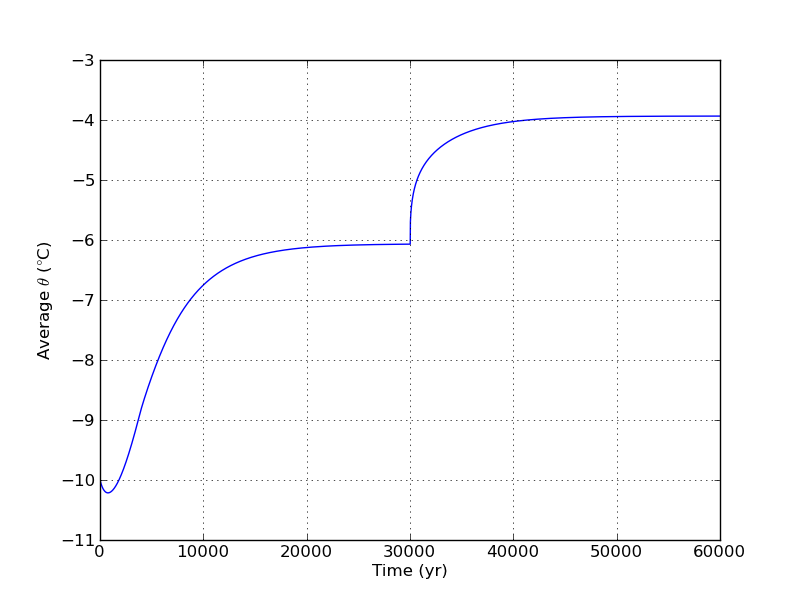
\includegraphics[width=0.42\textwidth]{images/60000yr_avg.png}
	\label{fig:500 year orbit}
	\caption{Average Temperature of Ice in 60,000 Years.}
\end{figure}

\noindent These data show that even though the surface temperature has increased by $15\ ^\circ C$, the average temperature of the ice has only increased $2\ ^\circ C$.

I made an investigation to find the precise value of $Q_{geo}$ to create a change of phase on the bed of the ice sheet and found that with \emph{any} value of $Q_{geo}$ with the depth of ice around 50 meters, the bed would eventually reach $\theta_{PMP}$ and incur a change of phase.  Once the ice temperature on the bottom gains any amount of heat, a chain reaction occurs which eventually brings the bottom temperature up to $\theta_{PMP}$, which for this depth is close to 0.  For increased ice thickness, the temperature on the bed could decrease without bound if $Q_{geo}$ was insufficient to overtake the horizontal velocity of ice.


%%Interpretation---------------------------------------------------------------
\section{Interpretation}
Creating this model provided a good deal of challenges.  Carefull examination of unit calculations was necessary, and a good deal of the work was based on theoretical concepts.  When plugging equations into a python script and testing results, errors would occur which were quite difficult to diagnose.  Creating this system required a good amount of courage to keep going forward and not to stop to check and re-check what I had already checked.

This model can be improved in a number of ways.  Accumulation rates on the surface and the rate of water runoff on the bed would provide better insight into the effects of increasing geothermal heat-flux.  If the water were able to escape from underneath the ice and no accumulation were to occur, a simulation could be made to determine the length of time and amount of energy needed to melt the entire ice sheet.

Although computationally expensive it would seem feasible to simulate multiple columns of ice simultaneously.  This would provide a view of the ice in a planar view and may be visualized as a vector-field.  A three-dimensional view of the ice-sheet may be useful if color-coded to show different heat patterns on the surface; a planar view of the inside of the ice which can be adjusted for depth would also be insightful.

With the correct equations and data regarding volcanoes, quite an interesting simulation could be performed.  Data could be obtained to determine the length of time needed preceding an eruption for an ice-sheet to repair itself.  A similar simulation regarding atomic weapons would also provide insight into theoretical worst-case scenarios.

I feel that a simulation of a subject is best accomplished when you can do \emph{anything} to the environment, and this project has brought me one step closer to understanding how that could be possible.


\end{document}
%%Compile with pdflatex file.tex



